\begin{figure}[t]
\centering
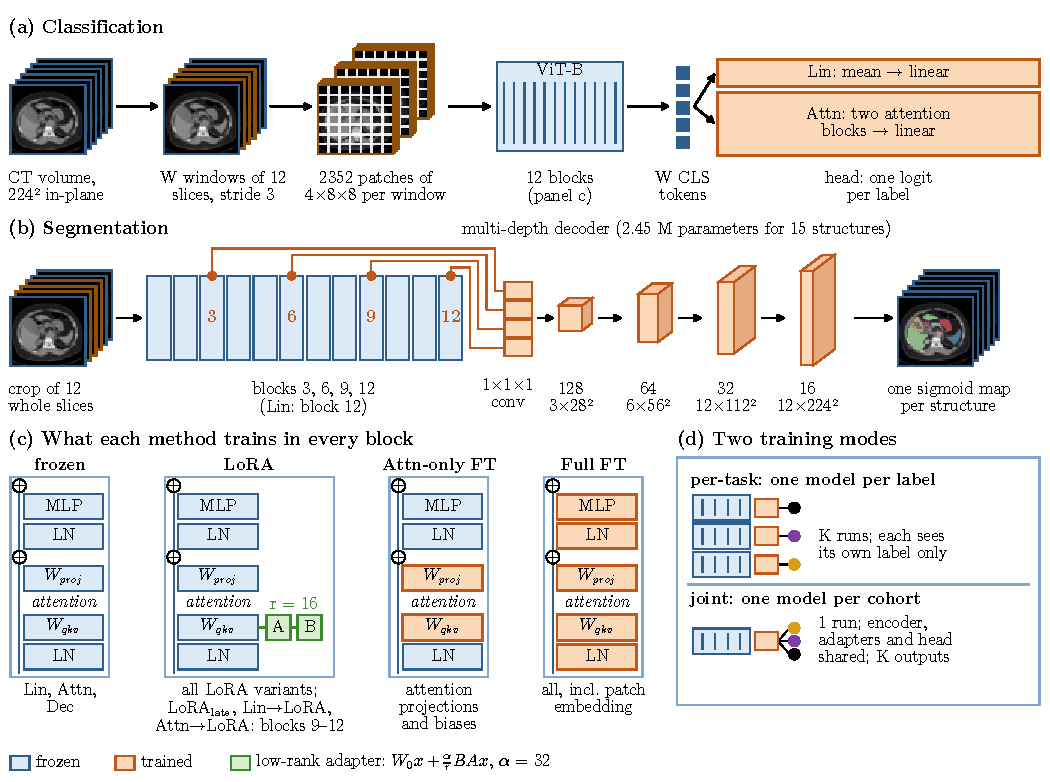
\includegraphics[width=\textwidth]{figures/fig_pipeline.pdf}
\vspace{-12pt}
\caption{How each task is run, shown for TAP-CT (other backbones: Figs.~\ref{fig:arms} and~\ref{fig:armsseg}, Appendix~\ref{app:details}). (a) Classification: the volume is split into $W$ 12-slice windows starting every 3 slices ($4\times8\times8$ patches), and the CLS token of every window enters the head, a linear layer on their mean (Lin) or an attentive probe (Attn), with one logit per label. (b) Segmentation: the tokens of blocks 3, 6, 9 and 12 feed a multi-depth decoder (2.45\,M parameters for 15 structures) with one sigmoid map per structure; Lin uses block 12 only. (c) Parameters each method trains in every encoder block; the head is always trained. (d) Per-task and joint training; in segmentation, a label is a structure and a cohort a dataset, and the 15-structure joint models train for three times the steps.}
\label{fig:pipeline}
\vspace{-5pt}
\end{figure}

\paragraph{Backbones.}\label{sec:backbones} First, \textbf{TAP-CT-B-3D} \citep{veenboer2025tapct} is a 12-block vision transformer pretrained using the DINOv2-style self-supervision on in-house CT (ViT-B; \citealp{dosovitskiy2021vit}), with $4\times8\times8$ voxel patches, a class (CLS) token, and four register tokens \citep{darcet2024registers}, applied to windows of $12\times224\times224$ voxels at native slice spacing (Fig.~\ref{fig:pipeline}). Second, \textbf{SPECTRE-Large} \citep{claessens2025spectre} is a 24-block ViT-L pretrained using self-distillation and vision-language alignment with radiology reports, with $16\times16\times8$ patches on $128\times128\times64$ crops, where for classification, 64 crops of a $512\times512\times256$ volume at $0.5\times0.5\times1$\,mm are summarized by its pretrained 4-block feature combiner. Third, Pillar-0 \citep{agrawal2025pillar0} is pretrained on CT and breast magnetic resonance imaging (MRI) data from a single academic center. We use its head-CT Atlas encoder, which comprises a convolutional stem followed by three stages of multi-scale window-attention blocks operating over the whole volume; given its head-CT specialization, we evaluate it only on RSNA19 ICH. Inputs follow each model's own orientation, spacing, and intensity normalization (Fig.~\ref{fig:arms} and Appendix~\ref{app:details}). We are among the authors of TAP-CT.

\paragraph{Classification Methods.}\label{sec:ladder} The methods differ only in which weights of each encoder block they train, among its attention, feed-forward (MLP) and layer-normalization (LN) weights (Figs.~\ref{fig:pipeline}c and~\ref{fig:arms}c). We analyze two \textit{types of probes} on the frozen features: \textbf{Lin}, a linear layer on a pooled feature, and \textbf{Attn}, an attentive probe \citep{bardes2024vjepa,chen2024cae} in which a learnable CLS token joins the window, crop or scale tokens and two self-attention blocks run over the set. We also test different \emph{low-rank adapters} on the query/key/value projections together with the attentive probe: \textbf{LoRA}, rank 16 ($\alpha=32$) on every block \citep{hu2022lora}; \textbf{LoRA$_{\text{late}}$}, on the last third of the blocks (for Pillar-0, its last stage, i.e., 8 of 12 blocks); \textbf{LoRA+ABMIL}, with tokens first pooled by gated attention-based multiple-instance learning (ABMIL; \citealp{ilse2018abmil}); \textbf{DoRA}, weight-decomposed LoRA \citep{liu2024dora}; and \textbf{rsLoRA}, rank-stabilized LoRA \citep{kalajdzievski2023rslora}, whose $\alpha/\sqrt{r}$ scaling is four times the LoRA scale at $r=16$. We also test \emph{two-stage schedules}: \textbf{Lin$\to$LoRA} and \textbf{Attn$\to$LoRA}, which train the probe for half the budget and then add late-block LoRA, keeping the probe's head \citep{kumar2022lpft}. Finally, for the \emph{full-rank fine-tuning (FT)} we have \textbf{Attn-only FT} which trains every parameter of the attention modules \citep{touvron2022three} and \textbf{Full FT} which trains every parameter of the encoder, together with the attentive head.

\paragraph{Segmentation Methods.}\label{sec:segmethods} For the segmentation tasks, we use the TAP-CT and SPECTRE backbones. We test two segmentation heads: \textbf{Lin}, which is a $1\times1\times1$ convolution on the deepest token grid, upsampled trilinearly, and \textbf{Dec} which is a light multi-depth decoder similar to UNETR \citep{hatamizadeh2022unetr} but without its skip connections from the input: the token grids of four depths are projected, concatenated, fused and upsampled to the voxel grid by $3^3$ convolutions (Figs.~\ref{fig:pipeline}b and~\ref{fig:armsseg}). \textbf{LoRA}, \textbf{LoRA$_{\text{late}}$} and \textbf{DoRA} add the adapters of classification under the multi-depth decoder, \textbf{Full FT} trains the encoder with it, and \textbf{Dec$\to$LoRA} trains Dec for half the budget before adding all-block LoRA. Predictions are independent sigmoid functions per structure.

\paragraph{Per-task and Joint Training.} Every cohort and dataset is trained in two modes with identical data and selection (Fig.~\ref{fig:pipeline}d): \emph{per-task}, where we have one model per label, and \emph{joint}, where we use one model with shared encoder, adapters and head and one output per label or structure. In this setup, we define a \emph{label-mode pair} as one label on one backbone in one of the two modes. Moreover, a per-task model has one output, whereas a joint model has one output per label or structure and sums the classification loss over the labels annotated for a case and it averages the segmentation loss over structures (Equations~\ref{eq:lcls} and~\ref{eq:lseg}, Appendix~\ref{app:details}).
